In any drone application, the drone's ability to react after an event is a key factor for the success of the application itself. 
In fact, we can see a drone application as an event-based system. 
In this kind of system, events (such as sensor readings, user inputs, or system states) trigger the execution of specific functionalities.

When developing a drone application, it is common to reason the solution following its event-based nature.
A general approach could be the definition of a set of tuples in the form \( \langle Event, Condition, Action \rangle \).
For example, suppose we need to implement the emergency landing feature of a drone application. 
In that case, we can model the solution with the tuple \( \langle GPS~signal~lost, Altitude~>~10m, Emergency~landing \rangle \).

In this chapter, we present EasyFly's Coordination Framework, a software component belonging to the ground station system meant to coordinate and orchestrate all the Crazyflie actions using an event-based system.
The Coordination Framework acts as a centralized entity that is able to synchronize different parts of the same application.

This approach encounters the developer's reasoning, allowing them to write the solution's implementation with less effort. 
Moreover, using the Coordination Framework, as we will see in the example at the end of the chapter (see Section~\ref{subsec:coordination_manager}), results in more descriptive and readable code.

In the following sections, we first present the role of this framework and its use cases, providing some concrete examples of possible applications. 
Then, we analyze its structure and design principles in detail.

\pagebreak% REASON FORMAT 
\section{The Role of the Coordination Framework}\label{sec:coordination_framework_role}

Coordination plays a crucial role in the successful implementation of drone applications. 
Depending on the application type, the coordination of a drone can be seen at two different levels:
\begin{itemize}
    \item Intra-drone coordination
    \item Inter-drone coordination
\end{itemize}

The first level of coordination considers the drone as an individual. 
In this case, coordination is considered to be the process of reacting in the face of a change in the surrounding environment or the drone's internal state with an ad hoc action properly defined.

In the case of intra-drone coordination, the role of the Coordination Framework is to watch over the current state of the drone (internal state or sensor data). 
When a specific condition is met, it performs the corresponding action.

A simple use case of the Coordination Framework considering intra-drone communication can be represented by the following:

\begin{displayquote}
    For the drone application that we are developing, we need the drone to be maintained not too close to the walls of the flight area. 
    Specifically, it must maintain a safe distance of 0,5 meters from the walls.
\end{displayquote}

In the use case scenario described above, we can model the solution using the following \( \langle Event, Condition, Action \rangle \) tuples:
\begin{enumerate}
    \item \( \langle Left~sensor~reading, Distance~<~0.5m, Move~right \rangle \)
    \item \( \langle Right~sensor~reading, Distance~<~0.5m, Move~left \rangle \).
    \item \( \langle Front~sensor~reading, Distance~<~0.5m, Move~backwards \rangle \).
    \item \( \langle Back~sensor~reading, Distance~<~0.5m, Move~forward \rangle \)
\end{enumerate}

The Coordination Managers can be used to transform the tuples defined into a real working application (see Section~\ref{subsec:coordination_manager}). 
In this case, the Coordination Managers, as the name suggests, will coordinate the defined actions, triggering them after the occurrence of the relative event and only if the condition is met.

From a more concrete point of view, the Coordination Framework will act as a supervisor entity that watches the values read by the drone's lateral proximity sensors. 
Whenever the distance is less than or equal to 0,5 meters, it will dispatch the action to move the drone in the opposite direction, bringing the distance from the wall back over the safe distance required.

Conversely, inter-drone coordination applies only to applications where the number of drones is more than one.
In these cases, the coordination is considered among individuals belonging to the same team.

By synchronizing the actions of multiple drones, coordination allows for the efficient and effective achievement of complex tasks that would be difficult or impossible for a single drone to accomplish alone. 
In this type of application, the role of the Coordination Framework is to watch over the state of the entire swarm and perform actions whenever a condition on the swarm state is met.

To make this concept of inter-drone coordination clearer, let's consider also in this case a simple use case:

\begin{displayquote}
    We need to develop a swarm drone application that performs simple choreography for a demonstration during a fashion event. 
    Our swarm is composed of three drones: D1, D2 and D3. 
    The choreographer designed the choreography: D1 starts flying and slowly increases its height to 1 meter from the ground. 
    After D1 completes its movement, D2 also starts flying and reaches a height of 0.5 meters. 
    When D2 has reached the target height of 0.5 meters, the drones D1 and D3 will slowly meet D2 at 0.5 meters from the ground. 
    Finally, to complete the choreography, land all the drones together.
\end{displayquote}\label{quote:simple_choreography}

In this use case scenario, the Coordination Framework needs to track the height of each swarm component.
For this reason, the swarm state will be represented by the tuple \( \langle D1~altitude, D2~altitude, D3~altitude \rangle \). 
Whenever the state changes, the Coordination Framework will decide on which actions to take according to the Table~\ref{table:inter_drone_use_case}

Also in this case, we can model the solution using the following \( \langle Event, Condition, Action \rangle \) tuples:
\begin{enumerate}
    \item \( \langle Swarm~state~changed,~~State = \langle 0, 0, 0 \rangle,~~D1~up~1m \rangle \)
    \item \( \langle Swarm~state~changed,~~State = \langle 1, 0, 0 \rangle,~~D2~up~0.5m \rangle \)
    \item \( \langle Swarm~state~changed,~~State = \langle 1, 0.5, 0 \rangle,~~D1~down~0.5m \rangle \)
    \item \( \langle Swarm~state~changed,~~State = \langle 1, 0.5, 0 \rangle,~~D3~up~1m \rangle \)
    \item \( \langle Swarm~state~changed,~~State = \langle 0.5, 0.5, 0.5 \rangle,~~land~all \rangle \)
\end{enumerate}

\begin{table}[tb]
    \centering
    \begin{tabular}{*{4}{|c}|}
    \hline
    \rowcolor{bluepoli!40}
    \textbf{D1 altitude} & \textbf{D2 altitude} & \textbf{D3 altitude} & \textbf{Action to take } \\
    \hline \hline
    0 & 0 & 0 & move D1 up to 1 meter \\
    \hline
    1 & 0 & 0 & move D2 up to 0.5 meter \\
    \hline
    1 & 0.5 & 0 & move D1 down and D3 up to 0,5 meter \\
    \hline
    0.5 & 0.5 & 0.5 & land all the drones \\
    \hline
    \end{tabular}
    \\[10pt]
    \caption{Use case scenario of inter-drone communication.}\label{table:inter_drone_use_case}
\end{table}

The key advantage of using this approach in both intra and inter-drone communication is that the entire business logic of the application is defined inside the Coordination Framework.
This fact implies that the only challenging task that the developer needs to take care of is the definition of the state and the relative actions to take when the state changes.
If the state is correctly updated and some external entity properly performs the actions defined, the Coordination Framework orchestrates all the stuff to achieve the application's goals correctly.

\section{Structure and Design Principles}\label{sec:coordination_structure_design}

The design structure of the Coordination Framework is a publish-subscribe architecture that follows the principle of the observer pattern.

The observer pattern is a design pattern in software engineering that defines a one-to-many relationship between entities,
where changes in one entity (the `observable` or `subject`) are automatically propagated to other entities (the `observers`) that depend on it.

In the observer pattern, the observable stores a list of observers and notifies them automatically whenever it changes state. 
This way, observers can take actions based on the observable's new state without constantly polling it for changes.

Following this design pattern, we designed the Coordination Manager considering four main actors:
\begin{itemize}
    \item \textit{Observable} -- Represents a state that can change over time.  
    
    \item \textit{Producer} -- The script/component that creates the Observable, providing an initial state. 
    Usually, this actor is in charge of updating the state of the Observable during time.

    \item \textit{Observer} -- The script/component interested in watching some Observables' changes. 
    Upon subscribing to the Observable, the Observer is notified by the framework when the former's state changes.

    \item \textit{Coordination Manager} -- It is the component in charge of managing the entire state of the drone application, allowing Producers to update the value of a portion of the state and notifying Observers whenever this happens.
\end{itemize}


\begin{figure}[tb]
    \centering
    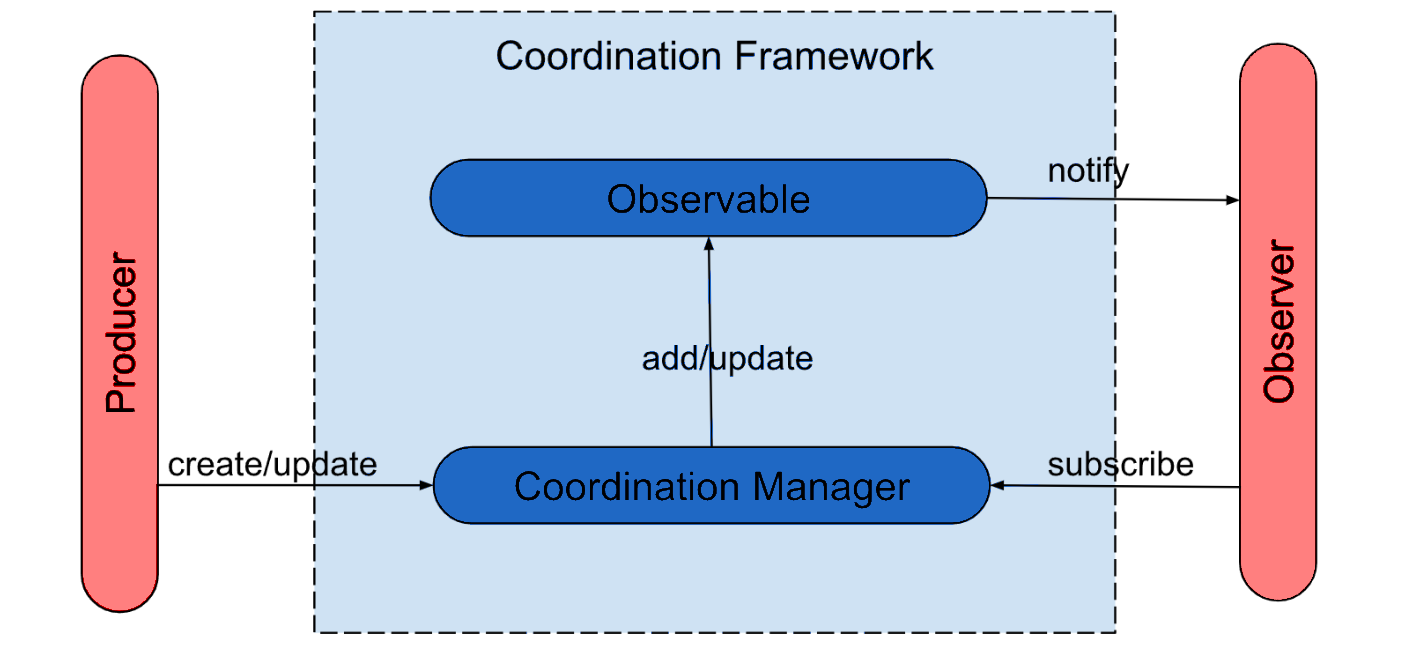
\includegraphics[width=0.9\textwidth]{coordination/design_architecture}
    \caption[The architecture of the Coordination Framework]{The architecture of the Coordination Manager comprises two internal entities: the Observable and the Coordination Manager. 
    Conversely, Producers and Observers are external to the framework and interact with it. }\label{fig:coordination_design_architecture}
\end{figure}

As presented in Figure~\ref{fig:coordination_design_architecture}, the core of the Coordination Framework is composed only of the Observable and the Coordination Manager entities.
The Producer and the Observer are entities considered outside the frameworks and only act as utilizers of its functionality.

\subsection{The Observable}\label{subsec:observable}
In our Coordination Framework, the Observable can be considered as the basic block of the entire structure.
In the core, the Observable holds a piece of information known as the state of the Observable. 

The state can be as complex as desired, and most importantly, it can change over time. 
Moreover, the state is atomic and cannot change partially; in other words, regardless of the complexity of the state, every update must provide complete information.

The Observable, on its own, is meaningless. 
It becomes valid only when an external entity (observer) is interested in watching the state and being notified when some update occurs.

For this reason, the Observable stores a list of references, known as subscriptions, to the external entities interested in watching the value of the state. 
In the standard observer pattern, the subscription consists of a callback function that the Observable uses to notify the Observer of the new value.
In our implementation, we decided to add some additional information to the subscription to increase the functionality of the pattern.
In particular, the subscription is a tuple composed of the following parts:
\begin{itemize}
    \item \textit{Action} -- A callback function to be called whenever the state of the Observable changes
    \item \textit{Condition} -- A predicate function that filters the values before notification. It is a function of the updated state of the Observable and decides whether to notify the Observer or not. 
    \item \textit{Context} --  It is an optional object to be passed as a parameter to the Action. It can contain some helpful information to allow the Observer to take the action. 
    When subscribing, the Observer can provide an arbitrary Context value; the provided Context will be stored in the subscription and sent back with each notification.
\end{itemize}

In the current implementations of the Coordination Framework, we have developed two types of subscriptions, one synchronous and the other asynchronous. 
As the names suggest, the synchronous subscription will block the execution of the Observer until the state is updated and the condition is satisfied.
Conversely, using the asynchronous subscription, the Observer will continue executing and be called back later when the value changes and the condition is met.

The standard observer pattern provides only the asynchronous notification. 
We decided to extend the pattern with the synchronous one also because, sometimes, it is useful to check that the drone application is in the desired state before continuing the execution.
An example of synchronous subscriptions becoming useful is the simple choreography example presented in Section~\ref{quote:simple_choreography}.
In that case, particularly if the swarm state can assume the same value at different times, triggering the right action at the right moment is essential.

To address that issue, we can adopt two possible solutions:
The first is to add one or more variables to the swarm state, with the drawback of introducing useless complexity and performance overhead.
The other more natural and simple solution is to wait for the execution of the events synchronously in the chronological order in which they have to appear.

To decide whether to use synchronous or asynchronous subscriptions, a general rule can be to use a synchronous subscription for events that occur only once and an asynchronous subscription for events that happen multiple times.

\subsection{The Coordination Manager}\label{subsec:coordination_manager}

\begin{figure}[tb]
    \centering
    \lstinputlisting[language=Python, caption={Wall avoidance navigation implemented using \textit{Communication and Coordination Frameworks}}, label=example_coordination]{Scripts/coordination_example.py}
\end{figure}

The Coordination Manager is the orchestrator of the entire Coordination Framework. 
Its role is to manage the whole application's Observables, creating and updating them when requested by some external Producer.

Its core is a global repository of Observables, representing the whole application state. 
Inside this repository, the Observables are identified by a unique name. 

As shown in Figure~\ref{fig:coordination_design_architecture}, the Coordination Manager represents the facade of the entire Coordination Framework; external entities like Producers and Observers are forbidden to manipulate the values stored inside the Observables directly.
This constraint allows centralized control, avoiding any possibility of an inconsistent state that may happen when different entities update the same portion of the state concurrently.

To better understand the working principle of the Coordination Framework, we can show in action the Coordination Manager explaining more in detail how the use case scenario described at the beginning of the chapter can be easily solved with this approach.
Listing~\ref{example_coordination} shows the script code that implements this solution. The scenario is the following:
\begin{displayquote}
    For the drone application that we are developing, we need the drone to be maintained not too close to the walls of the flight area. 
    Specifically, it must maintain a safe distance of 0,5 meters from the walls.
\end{displayquote}

As we have seen in the previous section, we can model the solution using the following \( \langle Event, Condition, Action \rangle \) tuples:
\begin{enumerate}
    \item \( \langle Left~sensor~reading, Distance~<~0.5m, Move~right \rangle \)
    \item \( \langle Right~sensor~reading, Distance~<~0.5m, Move~left \rangle \).
    \item \( \langle Front~sensor~reading, Distance~<~0.5m, Move~backwards \rangle \).
    \item \( \langle Back~sensor~reading, Distance~<~0.5m, Move~forward \rangle \)
\end{enumerate}

This reasoning helps us to define the State of the application. 
In particular, we can identify four Observables:
\begin{itemize}
    \item \textsc{Left Observable} -- representing the distance from left wall
    \item \textsc{Right Observable} -- representing the distance from right wall
    \item \textsc{Front Observable} -- representing the distance from front wall
    \item \textsc{Back Observable} -- representing the distance from back wall
\end{itemize}

To manage the updates of such a state, we can use the Communication Framework and setup one variable for each range direction (\textit{lines 16--18}).
After that, we can use the logging manager's notification system to add a watcher to each range direction (\textit{lines 20--24}).

Once we have defined the state and managed the update of such a state, then we can define the second part of the Coordination Manager.
To do this, we can set up 4 Observers(\textit{lines 26--32}), one for each Observable, to move the drone in the opposite direction of the wall (\textit{lines 8--9}).
Moreover, since we want to act only if the distance from one wall is less than 0.5 meters, we can specify for all the Observer a Condition function (\textit{lines 5--6}).


With this approach, the main advantage is that the entire business logic of the application is defined inside the Coordination Framework.
As the solution to the use case shows, this framework simplifies the task for a user, letting them focus on the definition of state and reactions instead of trying to manage all the coordination between the parts. 

Another advantage is that the resulting code is clean and can easily be read and understood also by users with less programming experience.
